\begin{figure*}[tp!]
	\begin{subfigure}{0.3\textwidth}
		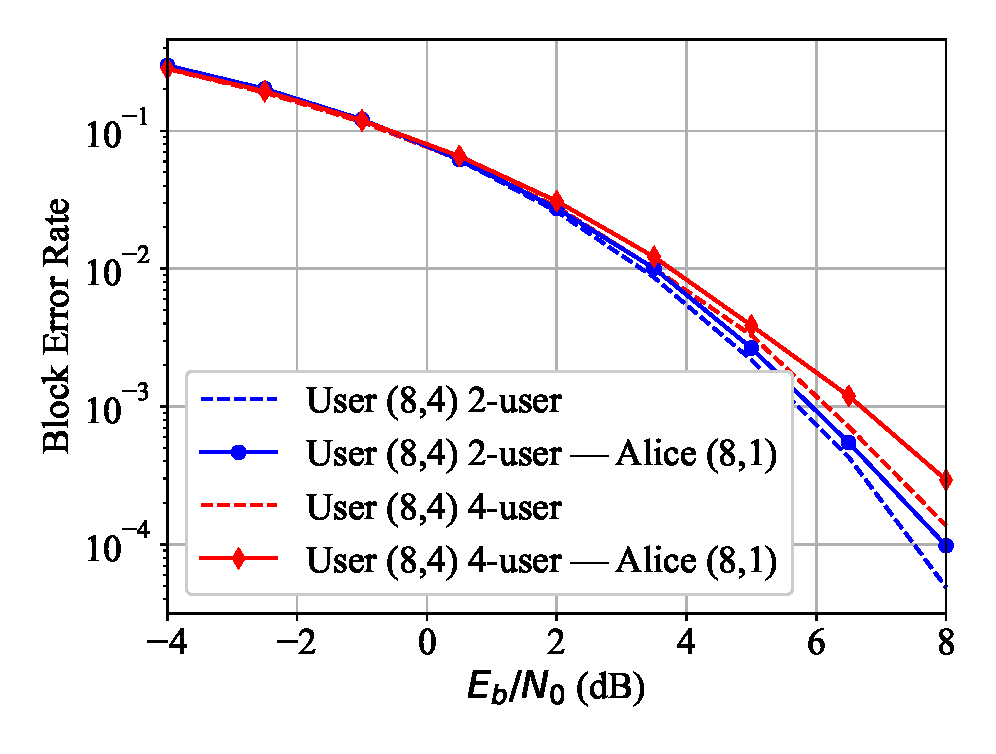
\includegraphics[width=\linewidth]{figs/multi_covert_autoencoder_bler_awgn}
		\caption{Autoencoder's BLER}
		\label{fig:multi_awgn_resutls_ae}
	\end{subfigure}
	\hspace*{\fill}
	\begin{subfigure}{0.3\textwidth}
		\includegraphics[width=\linewidth]{figs/multi_bob_bler_awgn}
		\caption{Bob's BLER}	
		\label{fig:multi_awgn_resutls_bob}
	\end{subfigure}
	\hspace*{\fill}
	\begin{subfigure}{0.3\textwidth}
		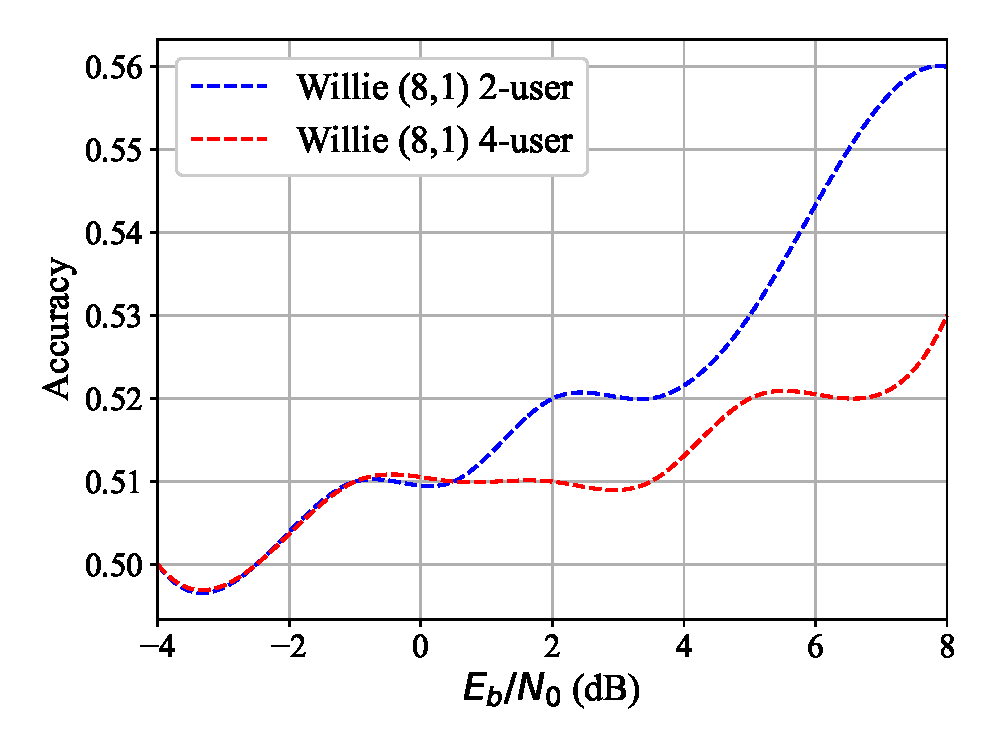
\includegraphics[width=\linewidth]{figs/multi_willie_accuracy_awgn}
		\caption{Willie's accuracy}	
		\label{fig:multi_awgn_resutls_willie}
	\end{subfigure}
	\caption{Trained covert models' performances over AWGN channel for systems with different numbers of users on a range of SNR values.}
	\label{fig:multi_awgn_results}
\end{figure*}
\begin{figure*}
	\begin{subfigure}{0.3\textwidth}
		\includegraphics[width=\linewidth]{figs/multi_covert_autoencoder_bler_rayleigh}
		\caption{Autoencoder's BLER}
		\label{fig:multi_rayleigh_resutls_ae}
	\end{subfigure}
	\hspace*{\fill}
	\begin{subfigure}{0.3\textwidth}
		\includegraphics[width=\linewidth]{figs/multi_bob_bler_rayleigh}
		\caption{Bob's BLER}
		\label{fig:multi_rayleigh_resutls_bob}	
	\end{subfigure}
	\hspace*{\fill}
	\begin{subfigure}{0.3\textwidth}
		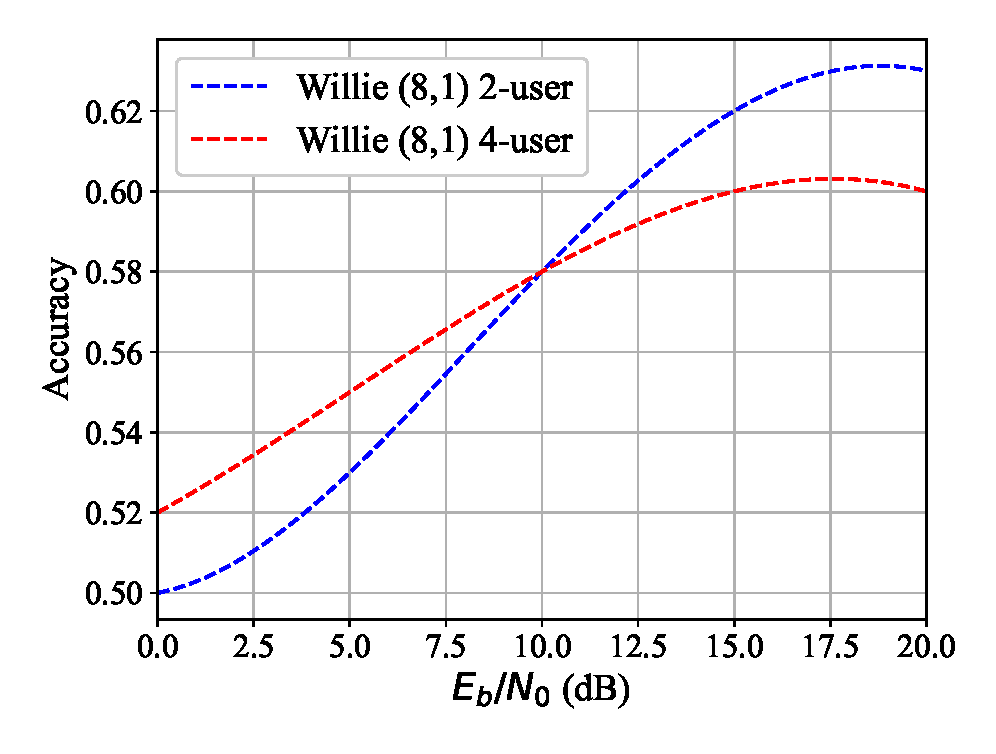
\includegraphics[width=\linewidth]{figs/multi_willie_accuracy_rayleigh}
		\caption{Willie's accuracy}
		\label{fig:multi_rayleigh_resutls_willie}
	\end{subfigure}
	\caption{Trained covert models' performances over Rayleigh fading channel for systems with different number of users on a range of SNR values.}
	\label{fig:multi_rayleigh_resutls}
\end{figure*}

\begin{table}[bp!]
	\begin{adjustbox}{width=0.9\columnwidth,center}
		\begin{tabular}{|l|l|} 
			\hline
			\multicolumn{2}{|c|}{\textbf{BaseRX Pre-decoder}}															\\
			\hline
			Layer 																	&	output dimension	\\														
			\hline
			Input & \(n_{tx}\) $\times$ 2 $\times$ 8 \\
			Dense + Tanh          													&	\(n_{tx}\) $\times$ 2 $\times$ 8		\\
			Convolutional (8 filters, kernel size 1 $\times$ 2, stride 1) + Tanh 	&   8 $\times$ (\(n_{tx}\) $\times$ 2 $\times$ 8 - 1)		\\
			Convolutional (8 filters, kernel size 1 $\times$ 4, stride 2) + Tanh 	&   8 $\times$ (\(n_{tx}\) $\times$ 8 - 2)		\\
			Convolutional (8 filters, kernel size 1 $\times$ 2, stride 1) + Tanh 	&   8 $\times$ (\(n_{tx}\) $\times$ 8 - 3)		\\
			Convolutional (8 filters, kernel size 1 $\times$ 2, stride 1) + Tanh 	&   8 $\times$ (\(n_{tx}\) $\times$ 8 - 4)		\\
			Dense + Tanh          													&	\(n_{tx}\) $\times$ 4 $\times$ 8		\\
			Dense + Tanh          													&	 \(n_{tx}\) $\times$ 4 $\times$ 8		\\
			\hline
			\hline
			\multicolumn{2}{|c|}{\textbf{BaseRX Decoders}}
			\\
			\hline
			Layer 																	&	output dimension	\\
			\hline
			Dense + Tanh															&	\(n_{tx}\) $\times$ 2 $\times$ 8		\\
			Dense + Softmax															&	16					\\ 
			\hline
			\hline
			\multicolumn{2}{|c|}{\textbf{Alice (AWGN)}} 															\\
			\hline
			Layer 																	&	Output dimension	\\
			\hline
			Input   											&	8 + $2^k$ \\ 
			Dense + ReLU          													&	32 + $2^{k+1}$		\\
			Dense + ReLU          													&	32 + $2^{k+1}$		\\
			Dense + ReLU   															&	8 $\times$ $2^k$	\\
			Dense + Tanh																	&	8 $\times$ 2	\\
			\hline
			\multicolumn{2}{|c|}{\textbf{Alice (Rayleigh)}} 															\\
			\hline
			Layer 																	&	Output dimension	\\
			\hline
			Input   											& 8 + $2^k$ + (\(n_{tx}\) $\times$ \(n_{tx}\) $\times$ 2)    	 		    \\ 
			Dense + ReLU          													&	32 + $2^{k+1}$ + (\(n_{tx}\) $\times$ \(n_{tx}\) $\times$ 2)	\\
			Dense + ReLU          													&	32 + $2^{k+1}$	\\
			Dense + ReLU   															&	8 $\times$ $2^k$	\\
			Dense + Tanh																	&	8 $\times$ 2	\\
			\hline
		\end{tabular}
	\end{adjustbox}
	\caption{BaseRX's  and Alice's networks details.}
	\label{table:autoencoder_structure}
\end{table}

\section{Evaluation of Multi-User Systems}
\label{s:multi_eval}
We break our multi-user system experiments into two different sections. First, we discuss the performance evaluation of our baseline autoencoder networks. Second, we will look into how our covert model performs when integrated into these models.


\subsection{Baseline Multi-User Autoencoders' Performance}
In section \ref{s:multi-model}, we noted that a multi-user autoencoder-based communication model is just an extension of the single-user model case. Notations used in this section are similar to that of section \ref{s:eval} subsection A. For all the transmitters of the system, we choose the numbers of channel uses \(n\) and the binary message of size \(k\) to be 8 and 4, respectively. There are two reasons for selecting these parameters in this way. First, it makes our results comparable to what is represented in \cite{o2017introduction} for multi-user systems as a baseline. Second, each user communicating at the half rate of BPSK makes the 2-user system results roughly comparable to a single-user system at the rate of BPSK, and the 4-user system to a single-user system at the QPSK rate. Nonetheless, our covert model is independent of these parameters and can be used for any autoencoder communication setup. Our datasets size and binary messages length are chosen to be the same as what we stated in \ref{s:eval}. Learning rate is set to 0.001 and the model is trained for 100 epochs. We use the Adam algorithm \cite{kingma2014adam} to optimize the parameters of our model and we set the batch size to 1024. For the channel configuration, we choose a fixed signal-to-noise ratio (SNR) value during training. In the case of the AWGN channel, we set the SNR to 8dB, and for Rayleigh fading channel that is 16db. Figure \ref{fig:multi_autoencoder_bler} shows the performance of our trained autoencoder-based communication models in terms of block error rate (BLER) for a range of SNR values under AWGN and Rayleigh fading channel models for different numbers of users. In both charts, 2-user and 4-user performances are depicted with blue and red colors, respectively and the results are compared with simulated traditional BPSK and QPSK systems with hard decision decoding.


\subsection{Covert Model Evaluation Results}
We evaluate our covert model's performance on two different channel models of AWGN and Rayleigh fading. They follow almost the same procedure to operate over both channel models except that Alice is fed with the channel matrix when the channel model is Rayleigh fading. In all experiments, covert users are set to transmit 1 bit of covert data over 8 channel uses. We integrate our covert model into both 2-User and 4-User systems to measure how the number of users would impact the overall model's performance. Since covert users' messages are embodied in the normal messages of other transmitters, we create the train and the test covert message \(m\) sets with the same size as the autoencoder's. All models are then jointly trained for 5000 epochs using the Adam optimizer. Importance of Alice's objectives are adjusted by setting \(\lambda_{Willie} = 2 \lambda_{Bob} = 4 \lambda_{UserRX}\) for AWGN and  \(4 \lambda_{Willie} = \lambda_{Bob} = 8 \lambda_{UserRX}\) for Rayleigh channel models in (\ref{alice_loss}). Just like our single-user model, we start the training with a learning rate of 0.001 and gradually halve the learning rate every 500 epochs. In each epoch, we first update the parameters of Willie's network using (\ref{willie_loss}), then train Alice's network for one step using (\ref{alice_loss}), and eventually optimize Bob's network based on (\ref{bob_loss}). Unlike training the autoencoder network, we find it better to train our covert models on a range of SNR values rather than a fixed value. That is, we set the SNR value to be in the range of 0dB to 12dB for the AWGN channel and 10dB to 25dB for the Rayleigh fading channel.


\begin{figure}[tp!]
	\center
	\begin{subfigure}{0.24\textwidth}
		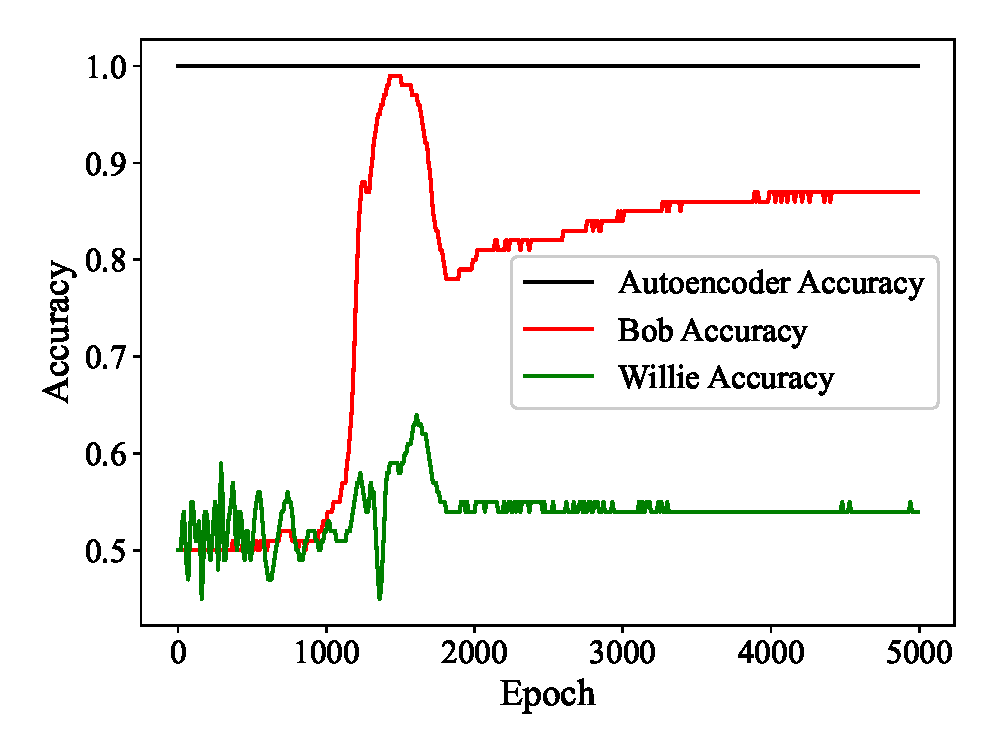
\includegraphics[width=\linewidth]{figs/multi_training_progress_awgn}
		\caption{AWGN channel}
	\end{subfigure}
	\hfill
	\begin{subfigure}{0.24\textwidth}
		\includegraphics[width=\linewidth]{figs/multi_training_progress_rayleigh}
		\caption{Rayleigh fading channel}	
	\end{subfigure}
	\caption{Evaluation results of our covert and autoencoder models during the training process show the system reaches a stable point after successful training.}
	\label{fig:multi_traning_progress}
\end{figure}


\textbf{Training Procedure}: In figure \ref{fig:traning_progress}, you can see the progress of each covert actor's accuracy on the test set during the training. It is evident from the plot that Bob gradually learns to decode covert messages \(m\) and establishes a working communication with Alice. Soon when the covert communication stabilizes, signals start to deviate from the distribution they had and this cause Willie to better tell them apart. When Willie's accuracy improves, the term \(\mathcal{L}_{Willie}\) dominates the other two objectives of Alice's loss function in (\ref{alice_loss}). Hence, Alice begins to gradually sacrifice its accuracy for covertness. These adjustments continue until the training process gets to a point where neither of the covert models improves no more. This will result in our models being successfully trained.


\textbf{Number of Users}: Figures \ref{fig:multi_awgn_results}, \ref{fig:multi_rayleigh_resutls} show our final model performances on two systems of 2-user and 4-user. It also demonstrates how numbers of users in the system affects our model's performance. Having more users in the system gives covert actors the ability to stay more covert. However, due to the system congestion, it will be more difficult for Alice and Bob to communicate reliably. More users' presence also causes heavier channel interference and consequently, we can see that covert users' impact on normal communications is slightly greater. Hence, it can be derived from the results that it becomes harder for covert models to establish a covert channel without impacting other users when there are already too many users in the system.


\textbf{Undetectibility}: In figures \ref{fig:multi_awgn_resutls_willie}, \ref{fig:multi_rayleigh_resutls_willie} we have visualized Willie's accuracy in percentage over a range of SNR values for classifying signals as normal and covert. These plots imply how probable it is for our covert signals to be detected by an observer at each SNR value. In both channel models, it is more probable for Willie to spot covert communication when there are fewer users in the system. We believe this is due to the more complex channel interference effect and noise model. When more users are communicating at the same time in the system, the distribution of channel effects becomes much more complex to learn for Willie.
